Es existieren verschiedene Quelloffene \acs{STUN}- und \acs{TURN}-Server. Ein bekannter, häufig verwendeter Server ist \glqq{}coturn\grqq{}. Coturn unterstützt sowohl die wichtigsten \acs{STUN}- (RFC3489, RFC5389), als auch \acs{TURN}-Spezifikationen (RFC5766). Zudem unterstützt Coturn die Authentifizierungsmaßnahmen der \glqq{}TURN-REST-API\grqq{}, welche das Erstellen von zeitlich limitierten Login-Daten zur Authentifizierung von Clients ermöglicht \cite{turnrestRFC}. Zur Relais-Datenübertragung unterstützt Coturn sowohl \acs{TCP}, als auch \acs{UDP}. Coturn ist zudem in den Repositories der verwendeten Linux-Distribution enthalten, was eine Installation erheblich vereinfacht.\par

\subsection{Installation}
Auf Ubuntu Version 18.04+ lässt sich der Server einfach über den Packetmanager \textit{apt} via der Kommandozeile installieren:
\lstset{style=STYLE_COMMAND_LINE_ARGUMENT_SINGLE_LINE}
\begin{lstlisting}[belowskip=-0.8 \baselineskip]
$ apt-get install coturn
\end{lstlisting}

Um den Server nach einem Systemneustart automatisch als System-Daemon zu starten, muss in der Datei \textit{/etc/default/coturn} die folgende Zeile geschrieben werden:
\lstset{style=STYLE_COMMAND_LINE_ARGUMENT_SINGLE_LINE}
\begin{lstlisting}[belowskip=-0.8 \baselineskip]
TURNSERVER_ENABLED=1
\end{lstlisting}

Der Server kann nun über den System- und Servicemanager \textit{systemd} gestartet, gestoppt oder neu gestartet werden:
\lstset{style=STYLE_COMMAND_LINE_ARGUMENT_SINGLE_LINE}
\begin{lstlisting}[belowskip=-0.8 \baselineskip]
$ systemd <start|stop|restart> coturn
\end{lstlisting}

\subsection{Konfiguration}
Die Server lässt sich über die Konfigurationsdatei \textit{/etc/turnserver.conf} konfigurieren. Die Konfiguration folgt einem Schlüssel-Wert Schema, getrennt durch ein Gleichheitszeichen. Der (gekürzte) Inhalt der Konfigurationsdatei ist in Abbildung~\ref{lst:coturnConfig} gelistet. Die Einstellungen werden in Tabelle~\ref{table:coturnConfig} näher erläutert.

\lstset{style=STYLE_COMMAND_LINE_ARGUMENT_SINGLE_LINE}
\begin{singlespace}
\begin{minipage}{\textwidth}
\begin{lstlisting}[caption={Coturn-Konfigurationsdatei -- turnserver.conf}, captionpos=b, label={lst:coturnConfig}]
listening-port=3478
listening-ip=0.0.0.0
external-ip=<external-ip>/<internal-ip>

min-port=10000
max-port=20000

use-auth-secret
static-auth-secret=<my-auth-secret>
realm=ba-webrtc.westeurope.cloudapp.azure.com

stale-nonce=0
fingerprint
\end{lstlisting}
\end{minipage}
\end{singlespace}

\begin{table}[ht]
\centering
\begin{tabularx}{\textwidth}{lX}
\toprule
Einstellung&Beschreibung\\

\midrule
listening-port&Der Port, auf welchem der Server auf Anfragen reagieren soll.\\
listening-ip&Ist dieser Wert gleich 0.0.0.0, so nutzt werden alle im System definierten IP-Adressen als Listening-Adressen verwendet.\\
external-ip&Die Externe IP-Adresse des Servers. Der Server befindet sich in einem Subnetz, daher wird auch die interne IP-Adresse benötigt.\\
min-port / max-port&Die Port-Reichweite, welche für Relais-Adressen verwendet werden kann.\\
use-auth-secret&Der Server soll die zeitlimitierte Authorisierungsmethode mit statischem Schlüsselwort verwenden (siehe: Authentifizierung).\\
static-auth-secret&Das statische Schlüsselwort zur Generierung von Passwörtern zur zeitlich limitierten Nutzung des Servers.\\
realm&Ein TURN-Server unterstützt verschiedene \glqq{}Realms\grqq{}, um Anfragen verschiedener Ursprünge untereinander zu isolieren. In diesem Fall wird nur ein \glqq{}Realm\grqq{} benötigt. Der Wert dieser Konfiguration ist bei Verwendung der TURN-REST-API jedoch nicht relevant, und kann einen beliebigen Wert enthalten \cite{turnrestRFC}.\\
stale-nonce&Ein Wert von 0 bewirkt, dass die Authentifizierung einer Sitzung nicht automatisch nach einiger Zeit ausläuft.\\
fingerprint&Fingerprinting von STUN- und TURN-Nachrichten soll für WebRTC standardmäßig aktiviert sein. Dies ist in der Konfigurations-Hilfsdatei von coturn definiert.\\
\bottomrule

\end{tabularx}
\caption{Erläuterung der Konfigurationsparameter.}
\label{table:coturnConfig}
\end{table}

\subsection{Authentifizierung}
Coturn bietet verschiedene Möglichkeiten, Nutzer zu authentifizieren, um eine Nutzung des Servers von Dritten, außerhalb des vorgesehenen Einsatzzwecks, zu limitieren:

\begin{itemize}
  \item \textbf{Statische Nutzerdaten}: In der Konfigurationsdatei können Nutzer-Passwort-Tupel statisch definiert werden. Diese Art der Authentifizierung ist einfach zu implementieren, allerdings in Situationen, in welchen die Nutzer die Zugangsdaten einfach auslesen können, ungeignet.
  \item \textbf{Dynamische Nutzerdaten}: Coturn kann Nutzerdaten aus einer Datenbank auslesen. In diese Datenbank können Nutzerdaten dynamisch eingefügt, oder entfernt werden.
  \item \textbf{TURN-REST-API}: Die TURN-REST-API verwendet geheime Schlüssel, welche zwischen einem Webserver und dem TURN-Server geteilt werden müssen. Der Webserver kann, basierend auf dem geheimen Schlüssel, dynamische, zeitlich limitierte Zugangsdaten generieren \cite{turnrestRFC}. Der Schlüssel kann statisch in der Konfigurationsdatei (\textit{static-auth-secret}) angegeben werden. Zudem ist es möglich, eine Reihe an Schlüsseln dynamisch in einer Datenbank zu definieren.
\end{itemize}

Für die Implementierung wird die TURN-REST-API verwendet, da diese kein Aufsetzen einer Datenbank vorraussetzt. Zudem eignen sich zeitlich limitierte Zugangsdaten hier gut, da die Anwendung einen praktisch öffentlichen Service bereitstellt, welcher von jedem Nutzer, welcher die Website aufruft, verwendbar sein soll. Da dafür kein Log-In notwendig sein soll, ist es nicht notwendig Nutzerdatenbanken mit personalisierten Zugangsdaten für jeden Nutzer zu erstellen.\par

\subsubsection{Zugangsdaten}
Zugangsdaten bestehen immer aus einem Nutzernamen und einem Passwort. Der Nutzername setzt sich aus einer Nutzer-ID und einem Timestamp zusammen \cite{turnrestRFC}. Die Form des Nutzernamen ist wie folgt vorgegeben:
\lstset{style=STYLE_COMMAND_LINE_ARGUMENT_SINGLE_LINE}
\begin{lstlisting}[belowskip=-0.8 \baselineskip]
timestamp:nutzerid
\end{lstlisting}

Der Timestamp ist der Ablaufzeitpunkt der Zugangsdaten, die Nutzer-ID kann beliebig gewählt werden, oder leer sein. Das Passwort ist der \acf{HMAC} aus dem Nutzernamen in der oben beschriebenen Form und dem geheimen Schlüssel. Als Hash-Funktion wird der \acf{SHA-1} verwendet. Zuletzt wird das Password in \textit{base64} encodiert. Ein Passwort lässt sich somit folgendermaßen generieren:
\lstset{style=STYLE_COMMAND_LINE_ARGUMENT_SINGLE_LINE}
\begin{lstlisting}[belowskip=-0.8 \baselineskip]
base_64(hash_hmac('sha1', nutzername, schluessel));
\end{lstlisting}

\subsubsection{Implementierung auf dem Webserver}
Die im vorherigen Unterpunkt beschriebene Generierung von Zugangsdaten wird vom Webserver übernommen. Tritt ein Spieler einem Raum bei und möchte sich unter Nutzung des STUN- und TURN-Servers mit weiteren Peers verbinden, so werden für diesen Nutzer spezifische, zeitlimitierte Zugangsdaten generiert.

\vspace{6pt}
\lstset{language=js, style=STYLE_CODE_JS}
\begin{singlespace}
\begin{lstlisting}[caption={Funktion zum Erstellen von Zugangsdaten -- utils.js}, captionpos=b, label={lst:maketurnstuff}]
const config = require('./config.json');
const crypto = require('crypto');
[...]
generateTURNCredentials : (user) => {
    const timestamp = Date.now() + config.ice.staticAuthCredentialLifetime;
    const username = `${timestamp}:${user}`;
    const hmac = crypto.createHmac('sha1', config.ice.staticAuthSecret);
    hmac.setEncoding('base64');
    hmac.write(username);
    hmac.end();
    const password = hmac.read();

    return [
      { urls: config.ice.stunServerAddress },
      { urls: config.ice.turnServerAddress, username: username, credential: password }
    ];
  },
}
\end{lstlisting}
\end{singlespace}

Die in Abbildung~\ref{lst:maketurnstuff} dargestellte Funktion generiert direkt ein Array an ICE-Servern mit zugehörigen Zugangsdaten, welche an den Client übertragen werden können. Der Nutzername (\textit{user}) ist dabei die ID des Client-Sockets, die Lebenszeit der Zugangsdaten ist in der Konfigurationsdatei des Webservers definiert. Der geheime Schlüssel (\textit{config.ice.staticAuthSecret}) muss mit dem in der Coturn-Konfigurationsdatei gesetzten Wert übereinstimmen.

\subsection{Ports}
Zuletzt müssen noch alle benötigten Ports freigegeben werden. Dazu kann das \textit{ufw (Uncomplicated Firewall)}-Werkzeug verwendet werden:
\lstset{style=STYLE_COMMAND_LINE_ARGUMENT_SINGLE_LINE}
\begin{lstlisting}[belowskip=-0.8 \baselineskip]
$ sudo ufw enable
$ sudo ufw allow <port>/<protocol>
\end{lstlisting}

Alle zu öffnenden Ports sind in Tabelle~\ref{table:ports} gelistet.

\begin{table}[ht]
\centering
\begin{tabularx}{\textwidth}{llX}
\toprule
Port&Protokoll&Beschreibung\\
\midrule
3000&TCP&Port des Webservers.\\
3478&TCP/UDP&Listening-Port des STUN- und TURN-Servers.\\
10000-20000&UDP&Ports für Relais-Adressen des TURN-Servers.\\
\bottomrule

\end{tabularx}
\caption{Portweiterleitung.}
\label{table:ports}
\end{table}

\begin{figure}[h]
\centering
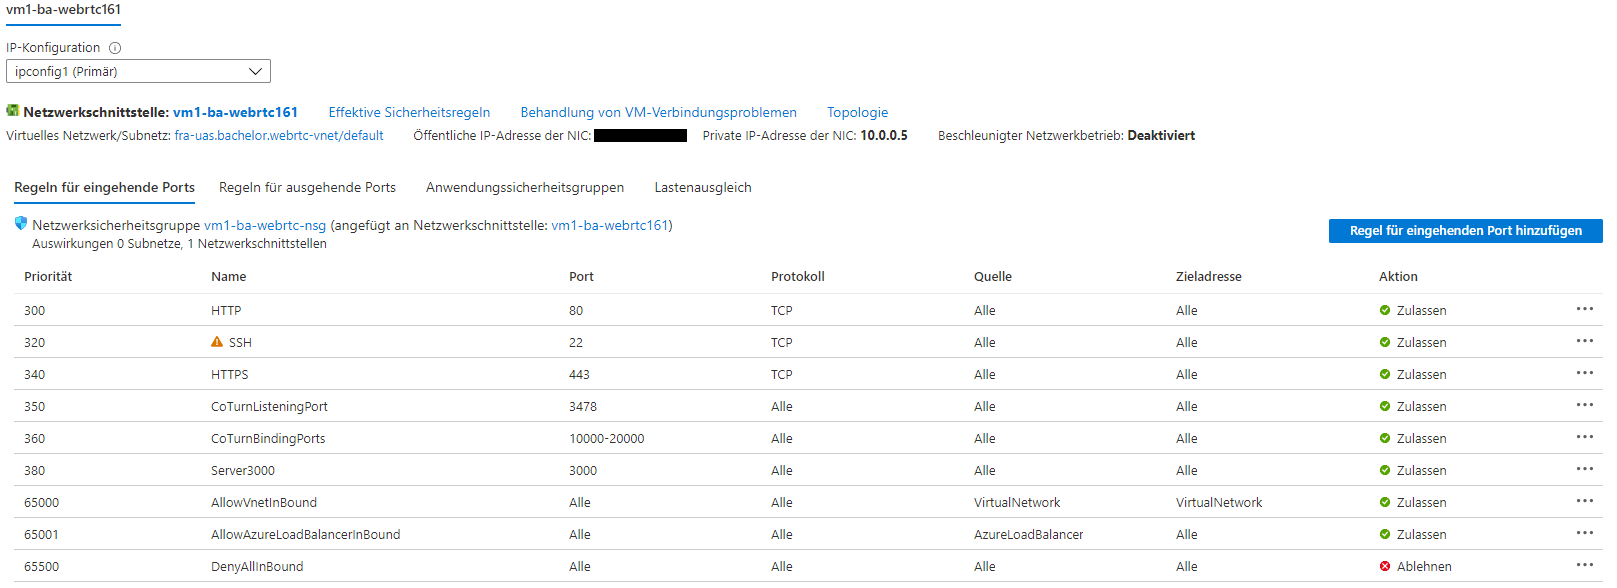
\includegraphics[width=0.95\textwidth]{bilder/azure-vm-network-config.png}
\caption{Port-Regeln der VM im Azure-Webportal.}
\label{fig:azurevmconfig}
\end{figure}

Die Ports müssen zudem für die \acs{VM} über das Azure-Webportal freigegeben werden. Dazu muss für jeden der Ports für die Ressource der VM im Unterpunkt \textit{Netzwerk} der Einstellungen eine Regel für eingehende Ports hinzugefügt werden (vgl. Abbildung~\ref{fig:azurevmconfig}).

\subsection{Test}
Um zu überprüfen, ob die STUN- und TURN-Server wie gewünscht funktionieren, müssen die vom ICE-Agenten einer RTCPeerConnection gefundenen ICE-Kandidaten geprüft werden. Wird eine neu erstellte RTCPeerConnection mit dem ICE-Server-Array konfiguriert, so werden bei Verbindungsaufbau die Folgenden ICE-Kandidaten (mit Ausnahme des \textit{host}-Kandidaten) gefunden:

\vspace{1pc}
\lstset{style=STYLE_ICE_CANDIDATE_0}
\begin{lstlisting}[caption={Relais-Kandidat},captionpos=b,label={lst:relaiskandidat}]
candidate:1411127089 1 udp 33562367 <@\textcolor{blue}{20.56.95.156}@> <@\textcolor{blue}{12926}@> <@\textcolor{red}{typ}@> <@\textcolor{red}{relay}@> raddr 0.0.0.0 rport 0 generation 0 ufrag uVtu network-cost 999
\end{lstlisting}

\vspace{1pc}
\lstset{style=STYLE_ICE_CANDIDATE_0}
\begin{lstlisting}[caption={Server-Reflexiver-Kandidat},captionpos=b,label={lst:srflxkandidat}]
candidate:842163049 1 udp 1677729535 <@\textcolor{blue}{(oeffentliche IP-Adresse)}@> <@\textcolor{blue}{55948}@> <@\textcolor{red}{typ}@> <@\textcolor{red}{srflx}@> raddr 0.0.0.0 rport 0 generation 0 ufrag QzUf network-cost 999
\end{lstlisting}

Die Transportadresse der Kandidaten ist jeweils in Blau, der Typ in Rot markiert. Beide Kandidaten werden gefunden. Der Port des Relais-Kandidaten liegt zwischen 10000 und 20000. Dies bestätigt, dass sowohl der STUN-, als auch der TURN-Server ansprechbar sind, und die Zugangsdaten korrekt sind.